
\chapter{Research question (Thesis chapter 3)}

% **************************** Define Graphics Path **************************
%\ifpdf
%    \graphicspath{{Chapter3/Figs/Raster/}{Chapter3/Figs/PDF/}{Chapter3/Figs/}}
%\else
%    \graphicspath{{Chapter3/Figs/Vector/}{Chapter3/Figs/}}
%\fi

%

\section{Estimate the impact of the new mechanism on the climatological mean state of the North Atlantic}

\subsection{ Hypothesis / Aim}
Develop a simple theoretical model of the findings in Part 1 and 2



%\begin{figure}	
%	\includegraphics[width=34pc,angle=0]{Y:/Code_Data/Plots_new/ECMWF/120104_maps/calcs/masksq_poly_time_diag-precip-msl_ens9_12012004.pdf}
%	\caption{Data}\label{fig:data}
%	\centering
%\end{figure}


\chapter {Research question (Thesis chapter3)} \label{Ch3}

%I will assess whether or not the warm path mechanism (Section 3.3), examined in the Met Office case study \cite{sheldon2017warm} and in section \ref{Ch2}, has relevance to the climatological state of the storm-track in the North Atlantic

I will examine the relationship between cyclone activity in the North Atlantic and the sea surface temperature in the Gulf Stream region. I will also estimate the impact of shear instability and slantwise convection on the climatological mean state of the North Atlantic. It is well established that many forecast busts over Europe are due to poor representation of atmospheric blocking \cite{rodwell2013characteristics}. It is also known that blocking and the state of the North Atlantic Oscillation (NAO) are related to storm track activity \citep{vallis2008local}. In this study, I propose that the small-scale mechanism of shear instability is a missing process in climate models, which can have a detrimental effect on the downstream forecast.

%
%Recent numerical experiments with high horizontal resolution (grid spacing of 25km or less) have suggested that the impact of the Gulf Stream on the “storm track” is mediated by the frontal circulation embedded in extra-tropical cyclones. In a series of controlled experiments with the UK Met Office Model, we were able to show that the frontal circulation can be destabilized by the Gulf Stream, with associated injection of low potential vorticity air at upper levels and a potential impact on blocking events further downstream, but we could not assess whether this effect was systematic (Sheldon et al., 2017). In this work, we address this issue by analysing an 11-member ensemble hindcast from ECMWF over the period 2007-2017 at a horizontal resolution of 16km. A large spread is found amongst ensemble members suggesting that, rather than systematically affecting the frontal circulation of cyclones, the effect of the Gulf Stream on them has to be understood within a statistical framework. 

\section{Aims}
\begin{itemize}
	\item Analyse operational forecasts, ensemble hindcasts and reanalysis run at ECMWF (1996 to present) using the shear instability diagnostic
	\item Explore the relationship between shear instability and state of the Gulf Stream
	\item Determine the impact of shear instability in extra-tropical cyclones on the downstream weather over western Europe
	\item Examine the upstream storm track activity (and shear instability) associated with forecast busts in terms of blocking indices
\end{itemize}


%Gerber and Valis 2009

%Unlike upright convection, slantwise convection transports air from low levels at one latitude to high levels at a different latitude. 

% http://www.atmo.arizona.edu/students/courselinks/spring16/atmo541b/handouts/pv_climo_bluestein1992.png

%\begin{figure}[h]
%	\centering
%	\noindent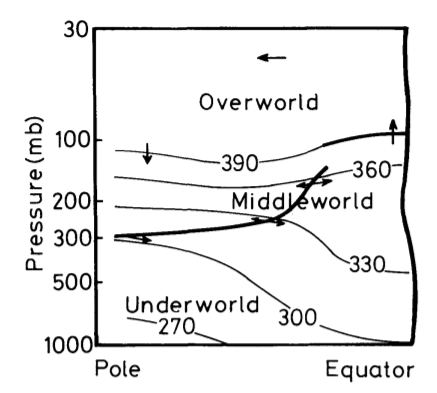
\includegraphics[width=18pc]{H:/Documents/Thesis/phd-thesis-template-2.2.2_AC/phd-thesis-template-2.2.2/Figs/Hoskins_PVview.png}
%	\caption{A schematic view of potential vorticity in the atmosphere. Isentropes every 30 K marked. Tropopause in thick black line. (what PV value?). The arrow indicate some boundaries. The equatorial boundary is defined by the zero PV contour. Source: \cite{hoskins1991towards}} \label{fig:PV_profile}
%\end{figure}

%Time series data downloaded 4th Oct https://www.esrl.noaa.gov/psd/gcos_wgsp/Timeseries/NAO/
%East Atlantic from http://www.cpc.ncep.noaa.gov/data/teledoc/ea.shtml
%Gulf Stream northern wall from PML http://www.pml-gulfstream.org.uk/data.htm

I will analyse hindcasts from 1996-2017 for DJF only. This data will come from hindcasts run on 26 dates (table \ref{t_winterdates}). To focus on the highest resolution sections of these runs (0.2$^0$), I will just retain the first 15 days.

\begin{table}[h]
	\caption{DJF hindcast dates 2016-2017. A total of 26 hindcast dates}\label{t_winterdates}
	\begin{center}
		\begin{tabular}{c}
			%	\begin{tabular}{cc}
			\hline\hline
			Mondays \\
			05/12, 12/12, 19/12, 26/12, 02/01, 09/01, 16/01, 23/01, 30/01, 06/02, 13/02, 20/02, 27/02 \\ 
			\hline
			Thursdays \\			
			01/12, 08/12, 15/12, 22/12, 29/12, 05/01, 12/01, 19/01, 26/01, 02/02, 09/02, 16/02, 23/02  \\ 			
			\hline
		\end{tabular}
	\end{center}
\end{table}

%There are 31 times and 20 years and levels 400, 500, 700. Interpolate to get level 600.
Figure \ref{t_winter_timeline} illustrates the many runs that will be analysed. At times there will be runs initialised on 5 different dates that are representing the same time, which will give 55 ensemble members.

\begin{figure}\label{t_winter_timeline}	
	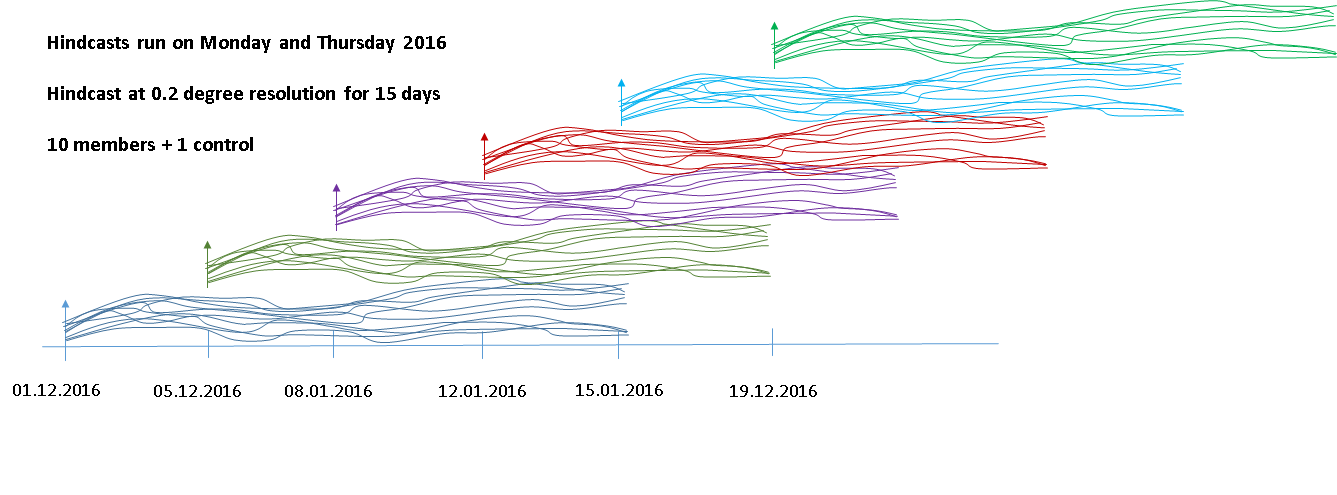
\includegraphics[width=34pc,angle=0]{H:/Documents/Thesis/phd-thesis-template-2.2.2_AC/phd-thesis-template-2.2.2/Figs/ecmwf_hindcast2.png}
	\caption{A section of the DJF 2016-2017 hindcast timeline. Hindcasts composed of 10 members plus one control are initialised on Mondays and Thursdays.}\label{fig:ecmwf_hindcast2}
	\centering
\end{figure}

As well as the ensemble hindcasts that are at 0.2$^0$ resolution, I will also analyse the operational control forecast, which has a different resolution depending on the year (see table \ref{t_ecmwf2}) along with the ERA-Interim renanalysis.
Using such a rich sample allows for both the climatology over a long time period to be examined, and also 
the ensemble spread on shorter timescales.


\section{Method}
Work has begun on downloading the large datasets required. I have also developed a working code for diagnosing atmospheric blocking based on the below.


\subsection{Atmospheric blocking indices}

A blocking time series has been calculated based on the method by \cite{davini2016northern}. To examine blocking over the Euro-Atlantic region, 60W-22.5W is the West Atlantic and 22.5W-45E is the East Atlantic.

$\phi_{0}$ = 60N; $\phi_{S}$ = 41.25N; $\phi_{N}$ = 78.75N; $\Delta$ = -3.75, 0, 3.75

\begin{equation} \label{eqblock1} %%% did not like blank line below - displaymath needs $$
GHGS(\lambda_{0}, \Delta) = \frac{Z500(\lambda_{0}, \phi_{0}+ \Delta) - Z500(\lambda_{0}, \phi_{S}+ \Delta)}
{\phi_{0} - \phi_{S}}
\end{equation}

\begin{equation} \label{eqblock2}
GHGN(\lambda_{0}, \Delta) = \frac{Z500(\lambda_{0}, \phi_{N}+ \Delta) - Z500(\lambda_{0}, \phi_{0}+ \Delta)}
{\phi_{N} - \phi_{0}}
\end{equation}


\begin{equation} \label{eqblock3}
IB(\lambda_{0}) = 1,   \textbf{if for any} \Delta ,  GHGS(\lambda_{0}, \Delta) > 0  , \textbf{and},   GHGN(\lambda_{0}, \Delta) < -5 m 
\end{equation}


This method, like many similar calculate the gradient in geopotential height (z) in a southern and northern region. If the gradient in the southern part is positive (i.e. increased westerlies) and in the northern part is negative (decreased westerlies), then blocking is diagnosed.
%Why 500 hPa?

% http://www.metoffice.gov.uk/learning/learn-about-the-weather/how-weather-works/factors-that-influence-uk-winters

%\begin{figure}[h]
%	\centering
%	\noindent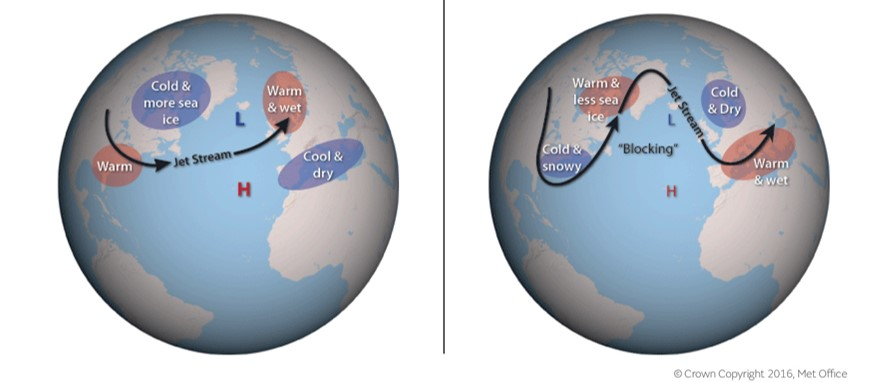
\includegraphics[width=38pc]{H:/Documents/Thesis/phd-thesis-template-2.2.2_AC/phd-thesis-template-2.2.2/Figs/nao_mo.jpg}
%	\caption{NAO}\label{fig:NAO}
%\end{figure}

A sector is considered blocked if at least 11.25 degrees in longitude is consistently blocked. A blocking event requires persistence in time of at least five consecutive days. Figure \ref{fig:block_criteria} shows the GHGS values for 2015. The red box in the bottom left hand corner illustrates the dimensions in time and space that must be satisfied in order for a blocking event to be categorised.
%NB Update plot to plot Hov of combined GHGS A and GHGNA???

\begin{figure}	
	\includegraphics[width=22pc,angle=0]{Y:/Code_Data/Chapter2_3/Plots/final/Hovm_GHGNA_2015_area.png}	
	\caption{Blocking event criteria in space and time}\label{fig:block_criteria}
	\centering
\end{figure}

%This blocking index has been calculated using... forecast ? hindcast?

%\begin{figure}
%		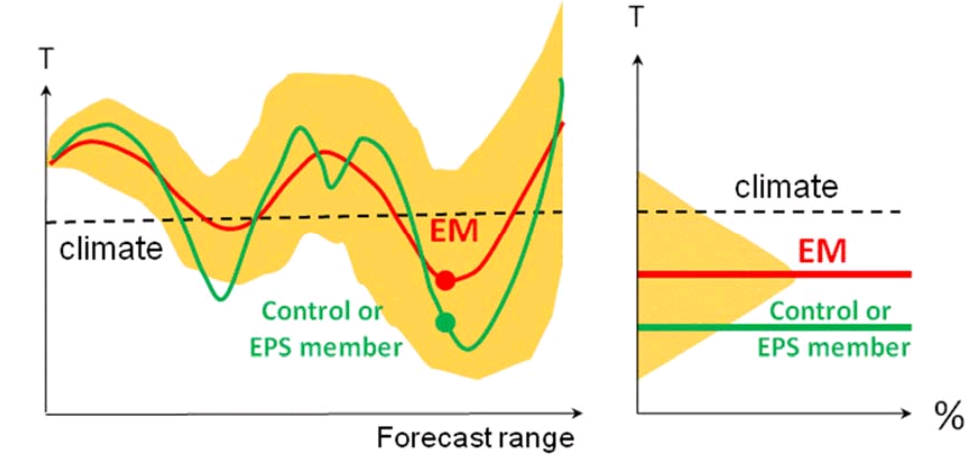
\includegraphics[width=22pc,angle=0]{H:/Documents/Thesis/phd-thesis-template-2.2.2_AC/phd-thesis-template-2.2.2/Figs/ens_spread.png}
%	\caption{Blocking events from ...}\label{fig:block_events}
%	\centering
%\end{figure}

%The period being examined initially is 2008-2017 DJF. 



\section{Possible future analysis across thesis chapters 2 and 3}

% https://software.ecmwf.int/wiki/display/CKB/What+is+ERA5

In Q2 2018 a new reanalysis produced by ECMWF will be released. ERA5 is the 5th major global reanalysis produced by ECMWF. Unlike ERA-Interim, which is deterministic, this reanalysis has 10 ensemble members, and also ensemble mean and spread for all parameters and levels are being produced. The horizontal resolution is considerably higher spatial and temporal resolution than its predecessor ERA-Interim: hourly analysis fields are available at a horizontal resolution of 31 km, and on 137 levels from the surface up to 0.01 hPa (around 80 km). In addition, information on uncertainties is provided for each parameter at 3-hourly intervals and at a horizontal resolution of 62 km.
Adding this reanalysis to the suite of data products analysed over a number of years alongside research for Chapter 3, as well as for the single storm analysis for Chapter 2 would be beneficial.
%79 km globally, 60 levels to 0.1 hPa31 km globally, 137 levels to 0.01 hPa
%10-member Ensemble of Data Assimilations (EDA) at 63 km resolutio





%%%%%%%%%%%%%%%%%%%%%%%%%%%%%%%%%%%%%%%%%%%%%%%%%%%%%%%%%%%%%%%%%%%%%
% APPENDIXES
%%%%%%%%%%%%%%%%%%%%%%%%%%%%%%%%%%%%%%%%%%%%%%%%%%%%%%%%%%%%%%%%%%%%%
%
% Use \appendix if there is only one appendix.
%\appendix

% Use \appendix[A], \appendix}[B], if you have multiple appendixes.
%\appendix[A]

%% Appendix title is necessary! For appendix title:
%\appendixtitle{}

%%% Appendix section numbering (note, skip \section and begin with \subsection)
% \subsection{First primary heading}

% \subsubsection{First secondary heading}

% \paragraph{First tertiary heading}

%% Important!
%\appendcaption{<appendix letter and number>}{<caption>} 
%must be used for figures and tables in appendixes, e.g.,
%
\newpage
\appendix
\chapter{Appendix}
%
%\section{Glossary}
%
%\subsection {Entropy (potential temperature)}
%Potential temperature is a more useful quantity than temperature as it is not affected my vertical movements - expansion and compression of air mass. Also most unstable path? requires no buoyancy. Calculated from temperature and pressure
%
%% used to use the brackets and backslash. Now use equation environment \[\theta =  T \big(\frac{P_0}{P}) ^{0.286} \]
%\begin{equation} \label{eq_theta}
%\theta =  T \big(\frac{P_0}{P}) ^{0.286}
%\end{equation}
%
%\subsection{Equivalent potential temperature:}  commonly referred to as theta-e ($\theta _{e}$), is a quantity that is conserved during changes to an air parcel's pressure (that is, during vertical motions in the atmosphere), even if water vapor condenses during that pressure change. It is therefore more conserved than the ordinary potential temperature, which remains constant only for unsaturated vertical motions (pressure changes). \\
%
%the temperature a parcel of air would reach if all the water vapor in the parcel were to condense, releasing its latent heat, and the parcel was brought adiabatically to a standard reference pressure, usually 1000 hPa (1000 mbar) which is roughly equal to atmospheric pressure at sea level. A thermodynamic quantity, with its natural logarithm proportional to the entropy of moist air, that is conserved in a reversible moist adiabatic process.
%
%
%\subsection{Potential vorticity:} the absolute circulation of an air parcel that is enclosed between two isentropic surfaces. If PV is displayed on a surface of constant potential temperature, then it is officially called IPV (isentropic potential vorticity). the product of absolute vorticity on an isentropic surface and static stability. So PV consists, in contrast to vorticity on isobaric surfaces, of two factors, a dynamical element and a thermodynamical element.
%
%\begin{equation} \label{eq_PV}
%
%PV = -g (\zeta + f)  \frac{\delta \Theta}{ \delta p} 
%
%\end{equation}
%
%The potential vorticity (PV) is the absolute circulation of an air parcel that is enclosed between two isentropic surfaces. If PV is displayed on a surface of constant potential temperature, then it is officially called IPV (isentropic potential vorticity). Of course, PV could also be displayed on another surface, for example a pressure surface. Note from the relation below, that PV is simply the product of absolute vorticity on an isentropic surface and static stability. So PV consists, in contrast to vorticity on isobaric surfaces, of two factors, a dynamical element and a thermodynamical element.

%
%\subsection{Hydrostatic:}
%The atmosphere is in hydrostatic balance when the upward pressure gradient force is balanced by the downward-directed gravitational pull of the Earth, or weight of the air column. On average the Earth’s atmosphere is  close to hydrostatic equilibrium, however, at high resolution (scales of 10 km or less), non-hydrostatic effects become relevant (ref ecmwf web and info from hydro vs non hydro).
%Two-time-level:
%
%Semi-implicit:
%
%Semi-Lagrangian: text book
%Correlation
%Correlation
%Covariance \\
